\documentclass[9pt,handout,serif]{beamer}
\usepackage{beamerthemeAmsterdam}
\usepackage{algorithm}
\usepackage{algpseudocode}
\usefonttheme{structuresmallcapsserif} 

%\usepackage{helvet}

%\documentclass[xetex,mathserif,serif]{beamer}
%\usetheme{Warsaw}

\title[Characterizing WLAN Channel Occupancy
for Cognitive Networking]%(optional, only for long titles)
{\textbf{Characterizing WLAN Channel Occupancy
for Cognitive Networking}}
%\subtitle{}
\author[Vizcaino Luna, A.] %
{A.~Vizcaino Luna \and \linebreak \linebreak Advisor: I. Glaropoulos \and \linebreak Examiner: V. Fodor}
\institute[Kungliga Tekniska Högskolan] % (optional)
{
  School of Electrical Engineering\\
  Kungliga Tekniska Högskolan
}
\date[2012] % (optional)
{June 2012}
\subject{Telecommuncation}

\begin{document}

\setbeamertemplate{headline}[tree] 
\begin{frame}
	\titlepage
\end{frame}

%\setbeamertemplate{headline}[tree]
\begin{frame}
	\frametitle{Table of Contents}
	\scriptsize
	%\tableofcontents[part=1,pausesections]
	\tableofcontents
\end{frame}

%Introduction
\section{Introduction}

\begin{frame}[c]
	\frametitle{Introduction}
	\begin{itemize}
		\item New wireless communication systems $\Rightarrow$ Scarcity of the wireless spectrum.
		\item Spectrum lightly used.
		\item Need of a control system for the interference between users of different systems.
		\item \textbf{Solutions:} orthogonality in space, frequency or \underline{time}.
		\item \textbf{Approach:} the take profit of the white spaces in the communications.
	\end{itemize}
\end{frame}

\subsection{Scenario}
\begin{frame}[c]
	\frametitle{Scenario}
	\begin{columns}
		\column{.5\textwidth}
		\textbf{WLAN}
		\begin{itemize}
			\item Highly common
			\item High Tx power
			\item High coverage
		\end{itemize}
		\column{.5\textwidth}
		\textbf{WSN}
		\begin{itemize}
			\item Low Tx power
			\item Limited detection range
			\item Resource/Hardware limited
		\end{itemize}
	\end{columns}
	
	\vspace{0.2in}
	
	\textbf{Problems:}
	\begin{itemize}
		\item High difference between Tx powers $\Rightarrow$ High interference
		\item WLAN terminals do not detect WSN transmissions
		\item WSN packets are usually long
	\end{itemize}
	\textbf{Solution:}
	\begin{itemize}
		\item Orthogonality in time: use of the white spaces in communications
		\item Necessity to model the WLAN traffic $\Rightarrow$ \textbf{semi-Markovian model}
	\end{itemize}
\end{frame}

\subsection{Topology}
\begin{frame}[c]
	\frametitle{Topology}
	\begin{figure}
		\includegraphics[width=0.4\textwidth]{../images/introduction/scenario}
	\end{figure}
	\textbf{WLAN}\\
	\begin{itemize}
		\item 802.11 IEEE
		\item Radius: 100 meters
		\item Transmit rate: 11 Mbps
		\item Transmit power: 15 dBm
	\end{itemize}
	\textbf{WSN}\\
	\begin{itemize}
		\item Cognitive access scheme with semi-Markovian model implemented
	\end{itemize}
	\textbf{Traffic Model}
	\begin{itemize}
		\item Multi-layer traffic model: session, flow and packet levels.
	\end{itemize}
\end{frame}

%Models
\section{Models}
\begin{frame}[c]
	\frametitle{}
	\begin{center}
		\textbf{\Huge{MODEL}}
	\end{center}
\end{frame}

\begin{frame}[c]
	\frametitle{Models}
	WLAN spectrum activity:
	\begin{figure}
		\includegraphics[height=0.3\textwidth]{../images/model/model}
	\end{figure}
	
	Two models under study
	\begin{itemize}
		\item \textbf{Global View Model:} ideal model. Unlimited sensing capabilities.
		\item \textbf{Local View Model:} real model. Limited sensing capabilities.
	\end{itemize}
	\textbf{Traffic Model:} multi-layer traffic model which includes session, flow and packet levels.
\end{frame}

\subsection{Global View Model}
\begin{frame}[c]
	\frametitle{Global View Model}
	\textbf{Ideal case:} the sensor has unlimited sensing capability. \\
	Two-state semi-Markovian simplifies the WLAN spectrum activity:
	\begin{figure}
		\includegraphics[width=0.2\textwidth]{../images/model/semi-markov_gv}
	\end{figure}
	Active distribution:
	\begin{equation}
		\label{eq:Active}
		f_A(t) = \frac{1}{\beta_{on} - \alpha_{on}}
	\end{equation}
	
	Mixture idle distribution:
	\begin{equation}
		\label{eq:Idle}
		f^{(CW)}_I(t) = \frac{1}{\alpha_{bk}}
	\end{equation}
	\begin{equation}
		\label{eq:Idle}
		f^{(WS)}_I(t) \triangleq \frac{1}{\sigma}(1+\xi\frac{t}{\sigma})^{(-\frac{1}{\xi}-1)}
	\end{equation}
	
	\begin{equation}
		\label{eq:Idle}
		f_I(t) \triangleq
		\begin{cases}
			p \, f^{(CW)}_I(t) + (1 - p) \, f^{(WS)}_I & t \le \alpha_{bk} \\
			p \, f^{(WS)}_I(t) & t > \alpha_{bk}
		\end{cases}
	\end{equation}
		
\end{frame}

\subsubsection*{Estimation}
\begin{frame}[c]
	\frametitle{Estimation}
	Active distribution:
	\begin{itemize}
		\item $\alpha_{on} \Rightarrow$ determined by the shortest active period.
		\item $\beta_{on} \Rightarrow$ determined by the longest active period.
	\end{itemize}
	Idle distribution:
	\begin{itemize}
		\item $\xi$ and $\sigma \Rightarrow$ determined by generalized Pareto distribution through Maximum-Likelihood Estimation.
		\item $p \Rightarrow$ determined by Uniform distribution through Moment Evaluation.
	\end{itemize}
\end{frame}

\subsection{Local View Model}
\begin{frame}[c]
	\frametitle{Local View}
	\textbf{Real case.} Limited sensing capabilities due to hardware limitations.	
	Three-state semi-Markovian model:
	\begin{columns}[c]
		\column{.5\textwidth}
			\begin{figure}
				\includegraphics[width=0.35\textwidth]{../images/model/LV_scenario}
			\end{figure}
		\column{.5\textwidth}
			\begin{figure}
				\includegraphics[width=0.8\textwidth]{../images/model/semi-markov_lv}
			\end{figure}
	\end{columns}
	
	Sensor skips part of the activity $\Rightarrow$ Mixture idle distribution no longer applicable.
	
	Active distribution: Uniform
	\begin{equation}
		f_A^{*}(t) = f_A(t)
	\end{equation}

	Idle distribution: combination of active seen/unseen + idle distributions.
	\begin{equation}
		f_{\bar{I}}^{*}=f_I^{*}(s)\frac{P_{cca}}{1-(1-P_{cca})f_I^{*}f_A^{*}}
	\end{equation}
	
\end{frame}

\subsubsection*{Estimation}
\begin{frame}[c]
	\frametitle{Estimation}
	Active distribution:
	\begin{itemize}
		\item $\alpha_{on} \Rightarrow$ determined by the shortest active period.
		\item $\beta_{on} \Rightarrow$ determined by the longest active period.
	\end{itemize}
	
	\vspace{0.2in}
	Idle distribution:\\
	\begin{itemize}
		\item $p_{cca}$ obtained with:
		\begin{equation}
			P_{cca} = \frac{\frac{p\alpha_{bk}}{2}+\frac{(1-p)\sigma}{1-\xi}+\frac{\alpha_{on}+\beta}{2}}{\frac{1}{N}\sum_{N}^{i=1}x_i+\frac{\alpha_{on}+\beta}{2}}
		\end{equation}
		\item $\xi$, $\sigma$ and $p$ obtained through Laplace estimation.
	\end{itemize}
\end{frame}

\subsubsection*{Laplace Estimation}
\begin{frame}[c]
	\frametitle{Laplace Estimation}
	Based on minimization of MSE.\\
	\begin{itemize}
		\item State space:
		\begin{equation}
			K = \{K_0, K_1, ..., K_n\}
		\end{equation}
		\begin{equation}
			K_n = (\xi_n, \sigma_n, p_n)
		\end{equation}
		\item Discrete space for $\xi, \sigma, p$ parameters.
		\item Minimization of the MSE:
		\begin{equation}
			arg min MSE(N; K_n) = arg min \frac{1}{s}\sum_{S}^{k=0}(f_{Ie}^{*}(s;N)-f_I^{*}(s;K_n))^2
		\end{equation}
	\end{itemize}
	Algorithm:
	\begin{enumerate}
		\item Select state $K_i = (\xi_i, \sigma_i, p_i)$
		\item \textbf{if} $MSE(N_i, \xi_i, \sigma_i, p_i) > MSE(N_j, \xi_j, \sigma_j, p_j)$
		\item Return the most popular state
	\end{enumerate}
\end{frame}

%\subsubsection*{Laplace Estimator}
%\begin{frame}[c]
%		\frametitle{Laplace Estimation}
%		\scriptsize
%		\begin{algorithmic}	
%			\item [\textbf{Step 0:}] \\
%					Choose randomly a starting state $K_0 \epsilon \textbf{K}$.
%					\hspace{1.5em} \State $Q_0(K_0) \gets 1 $ and $Q_0(K_n) \gets 0 $, $\forall K_n  \epsilon K$, $K_n \neq K_0$.
%					\hspace{1.5em} \State $m \gets 0$ and \State $K^{*}_m \gets K_0$.\\
%					Go to Step 1.
%			\item[\textbf{Step 1:}] \\
%					Generate a uniform random variable $J_m$ such that for all $K_n \epsilon K$, $K_n \neq K_0$, $J_m \gets K_n$ with probability $\frac{1}{K-1}$. \\
%					Go to Step 2.
%			\item[\textbf{Step 2:}] \\
%					Generate an observation $R_m$ of $Z_{lm}^{K_m \gets J_m}$.
%				\If	{$R_m > 0$} \\
%					\hspace{1.5em} $K_{m+1} \gets J_m$.
%				\Else \\
%					\hspace{1.5em} $K_{m+1} \gets K_m$.
%				\EndIf \hspace{1.5em} Go to Step 3.
%			\item[\textbf{Step 3:}] \\
%					$m \gets m + 1, Q_m(K_m) \gets Q_{m-1}(K_m) + 1$ and $Q_m(K_n) \gets Q_{m-1}(K_m)$ for all $K_n \neq K_m$.
%					\If {$Q_m(K_m) > Q_m(K_{m-1}^{*})$}
%						\hspace{1.5em} $K_m^{*} \gets K_m$.
%					\Else \\
%						\hspace{1.5em} $K_m^{*} \gets K_{m-1}^{*}$
%					\EndIf \hspace{1.5em}\\
%					Go to Step 1.
%	\end{algorithmic}
%\end{frame}

\subsection{Model Validation}
\begin{frame}[c]
	\frametitle{Kolmogorov-Smirnov}
	\begin{itemize}
		\item Kolmogorov-Smirnov validation test for fitting empirical-estimated distributions.\\
		\item Pseudo-code for implementation:\\
	\scriptsize
	\begin{algorithmic}
		\item[1] Add idle samples only if $t_{sample} > alpha_{BK}$
		\item[2] Find the maximum deviation between the empirical and estimated distributions
			\hspace{1.5em} \For {$i$ in {$1..\#samples$}} \\
				\hspace{1.5em} Find CDF of sample $i$. \\
				\hspace{1.5em} $d = max(abs(\frac{j}{n} - sample_{CDF}), d)$
			\EndFor
		\item[3] Estimate the P-value.
			\hspace{1.5em} \For {$i$ in {$1..\#runs$}} \\
				\hspace{1.5em} Generate $N = \#samples$ uniformly distributed values. \\
				\hspace{1.5em} $D = max(abs(\frac{j}{n} - value_{CDF}), D)$
				\If {D >= d} \\
					\hspace{1.5em} $count++$
				\EndIf
			\EndFor
		\item[4] Return D and P values. \\
			$P = count/\#runs$.				
	\end{algorithmic}
	\end{itemize}
\end{frame}

\subsection{Traffic Model}
\begin{frame}[c]
	\frametitle{Multi-layer traffic model}
	Multi-layer traffic model based on three levels: session, flow and packet.
	\begin{figure}
		\includegraphics[width=0.5\textwidth]{../images/model/TrafficFlow}
	\end{figure}
	Different distributions to model each level:
	\begin{table}
	\begin{center}
		\begin{tabular}{ l | c | c }
			Modeled Variable & Distribution & Parameters \\ \hline
			Session inter-arrival & Poison & min = 1, max = 928, median = 11\\
			Flow number & Bi-Pareto & $\alpha = 0.07$, $\beta = 1.75$, $c = 295.38$, $k = 1$\\
			Flow inter-arrival & Log-normal & $\mu = -1.6355$, $\sigma = 2.6286$\\
			Flow size & Bi-Pareto & $\alpha = 0.00$, $\beta = 1.02$, $c = 15.56$, $k = 111$\\
		\end{tabular}
	\end{center}
\end{table}
\end{frame}

%Simulation
\section{Simulation}

\begin{frame}[c]
	\frametitle{}
	\begin{center}
		\textbf{\Huge{SIMULATION}}
	\end{center}
\end{frame}

\subsection{Software}
\begin{frame}[c]
	\frametitle{Simulation}
	\begin{itemize}
		\item Network Simulation 2 + NS-Miracle: open-source discrete event simulator of networks with TCP, routing and multicast protocols support.
		\item "dei80211mr": library for the 802.11 protocol over NS2.
		\item Multi-layer traffic model C++/GSL library: bi-Pareto, Log-normal, uniform and exponential random distributions.
		\item Protocol Stack:
			\begin{figure}
				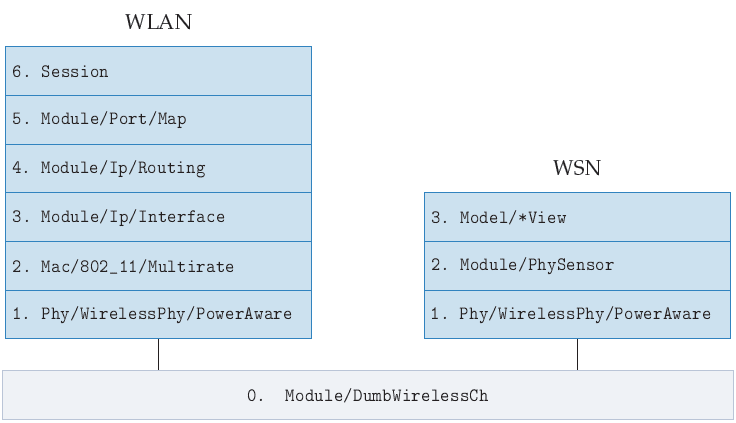
\includegraphics[width=0.5\textwidth]{../images/simulation/protocol_stack}
			\end{figure}
	\end{itemize}
\end{frame}

%Results
\section{Results}

\begin{frame}[c]
	\frametitle{}
	\begin{center}
		\textbf{\Huge{RESULTS}}
	\end{center}
\end{frame}

\subsection{Global View}
\begin{frame}[c]
	\frametitle{Global View Experiments}
	\begin{itemize}
		\item Study of the extraction of the idle distribution
		\item Idle distribution sensitivity
		\item Estimation process
		\item Model Validation
		\item Autocorrelation study of the idle periods for the KS test
		\item Effect of the number of samples in the Kolmogorov-Smirnov Validation test
		\item Session and in-session experiments
	\end{itemize}
\end{frame}

\subsubsection*{Study of the extraction of the idle distribution}
\begin{frame}[c]
 	\frametitle{Study of the extraction of the idle distribution}
	Mixture idle distribution composed by:
	\begin{itemize}
		\item Uniform distribution: $[0 < t < \alpha_{bk}]$
		\item Genearlized Pareto distribution: $[t > \alpha_{bk}]$
	\end{itemize}
	\begin{figure}
		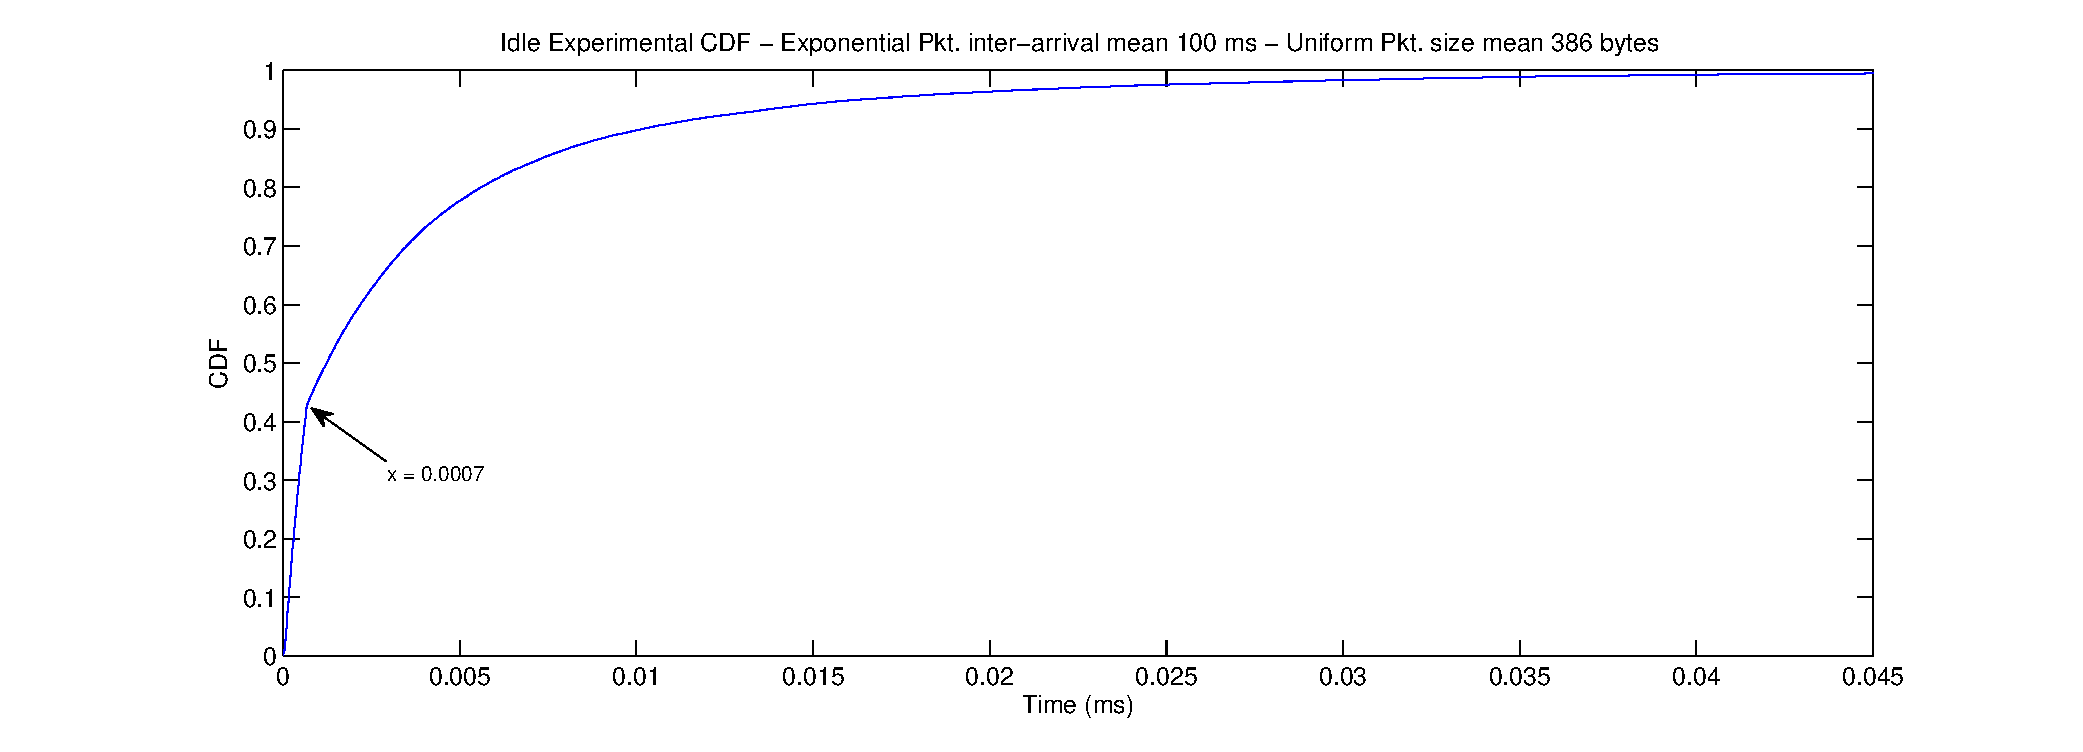
\includegraphics[width=\textwidth]{../images/results/GlobalView/cdf_globalview}
	\end{figure}
	Two clear different areas in the idle distribution CDF.
\end{frame}

\subsubsection*{Idle distribution sensitivity}
\begin{frame}[c]
	\frametitle{Idle distribution sensitivity}
	Test the idle distribution for different active and idle distributions.
	\begin{center}
	\begin{columns}
		\centering
		\column{.5\textwidth}
			\begin{figure}
				\centering
				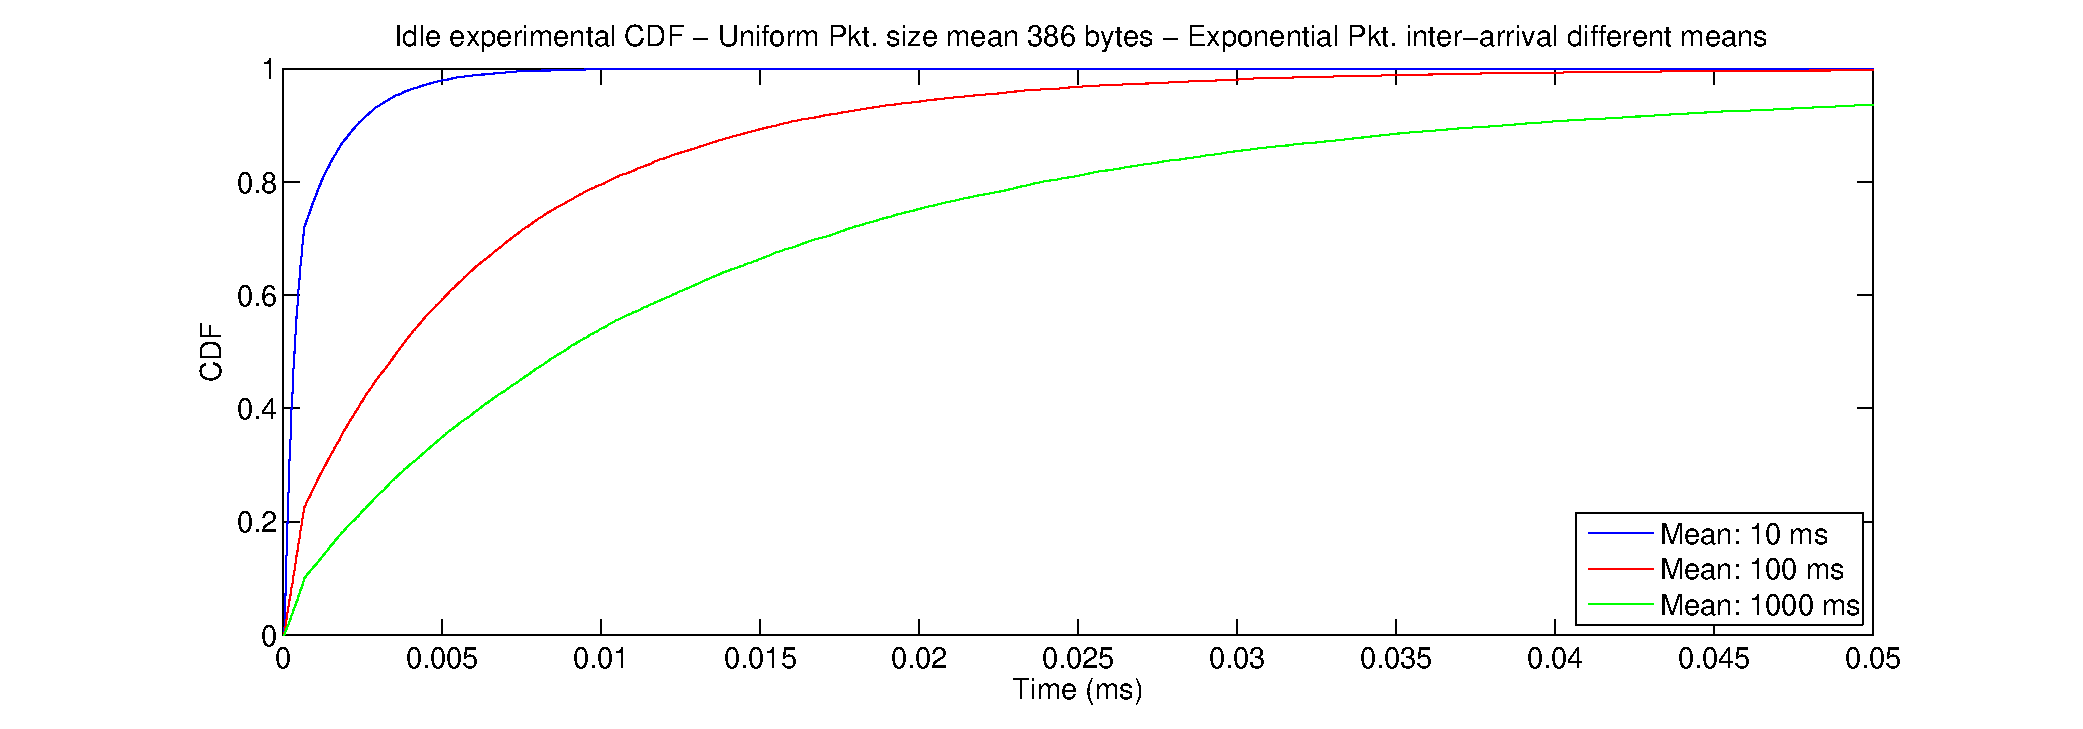
\includegraphics[width=1.1\textwidth]{../images/results/GlobalView/cdf_exponential}
			\end{figure}
		\column{.5\textwidth}
			\begin{figure}
				\centering
				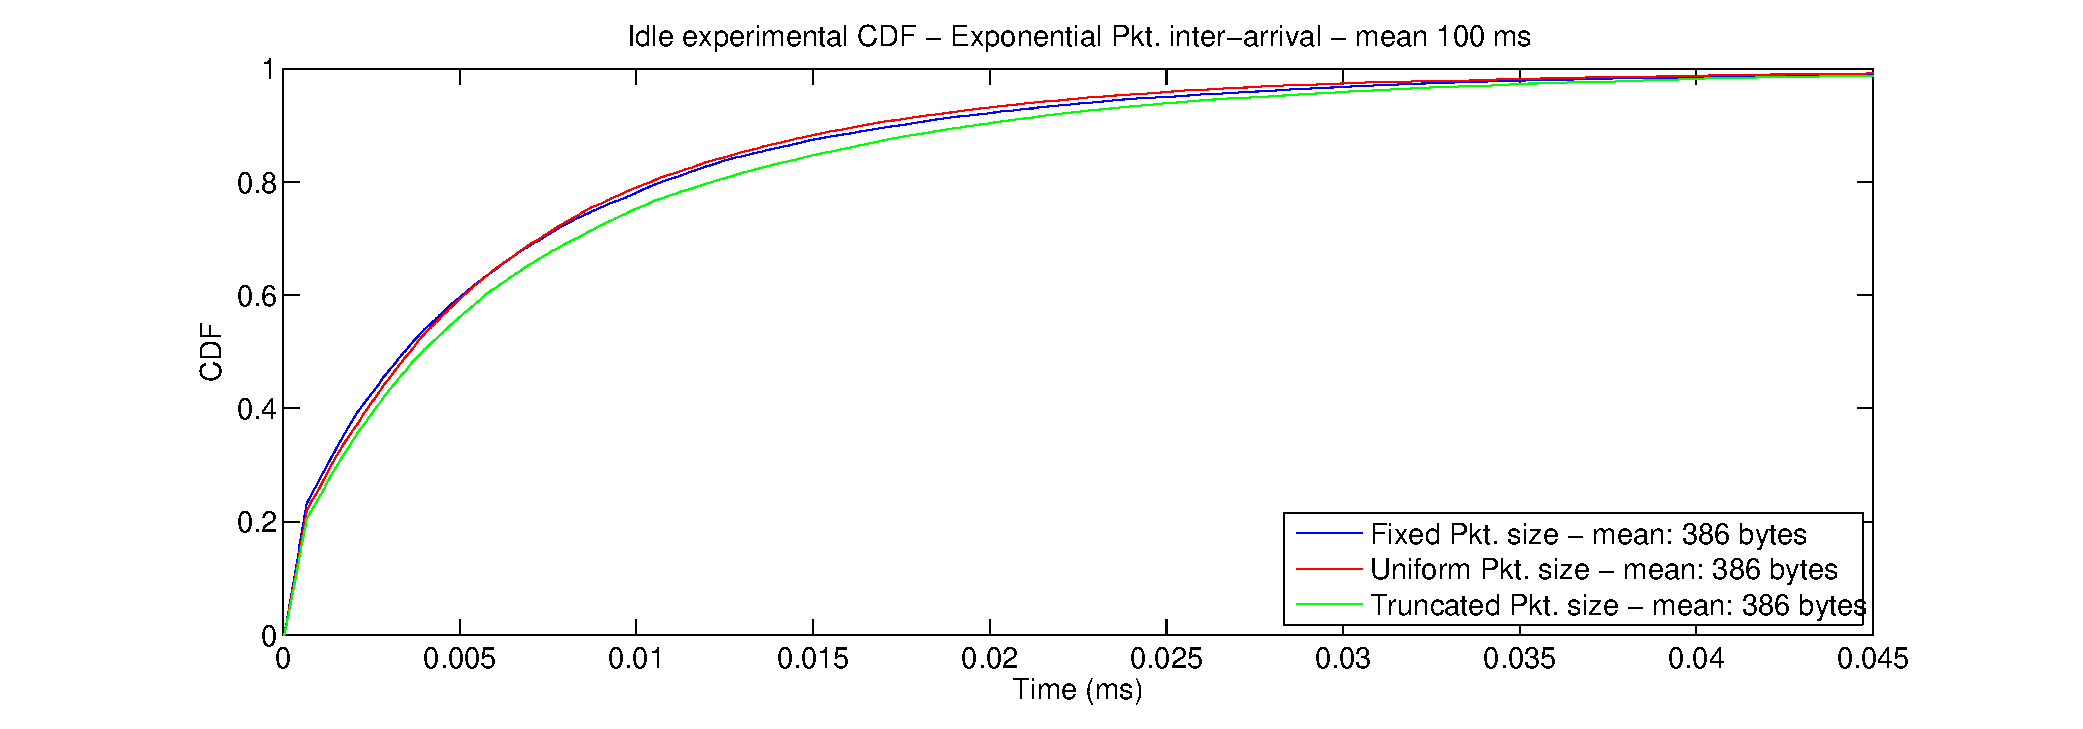
\includegraphics[width=1.1\textwidth]{../images/results/GlobalView/cdf_pkt_sizes}
			\end{figure}
	\end{columns}
	\end{center}
	\begin{figure}
		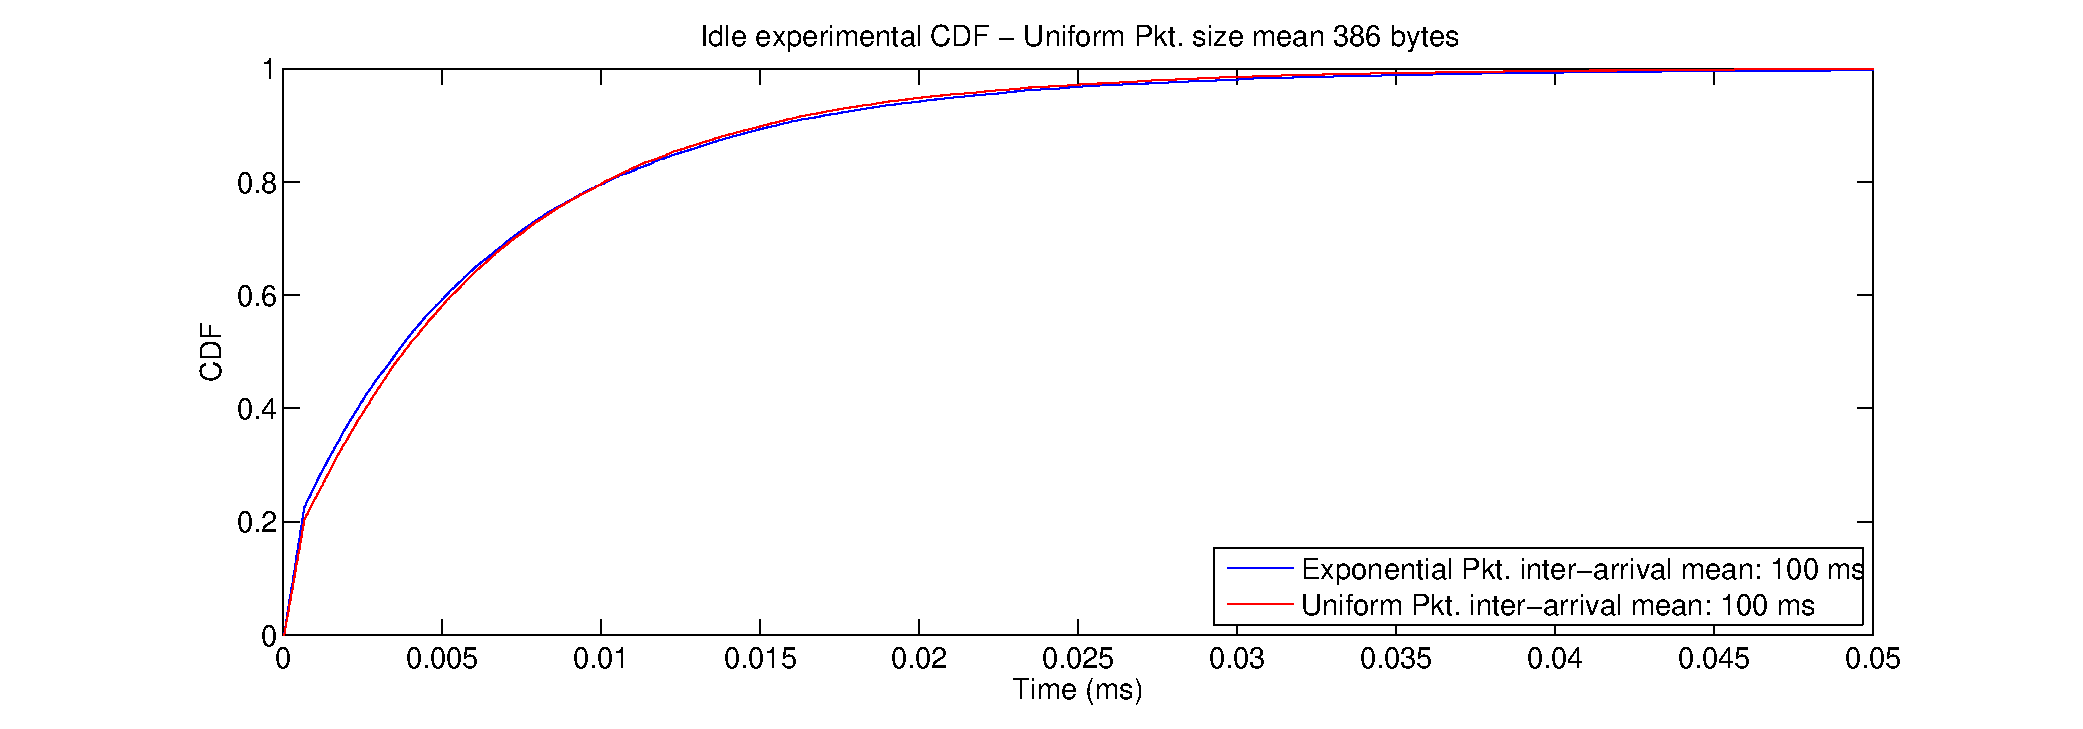
\includegraphics[width=0.6\textwidth]{../images/results/GlobalView/cdf_idle_same_mean}
	\end{figure}
\end{frame}

\subsubsection*{Estimation process}
\begin{frame}[c]
	\frametitle{Estimation Process}
	\begin{itemize}
		\item Testing of the Maximum-Likelihood estimation process for different traffic scenarios.
		\item Session number, flow number, sizes and inter-arrivals are fixed for all the tests.
		\item Packet sizes and inter-arrivals are randomized.
		\item The estimated parameters from the MLE process should not differ for different runs of the same scenario configuration.		
	\end{itemize}
	
	\begin{table}
	\centering
	\begin{tabular}{ c | c | c }
		& Mean & Std. Deviation \\ \hline
		$\xi$ & 0.117043 & 0.011688 \\ 
		$\sigma$ & 0.00610565 & 8.42259e-05 \\
		$p$ & 0.134211 & 0.00375842 \\
	\end{tabular}
	\end{table}
\end{frame}

\subsubsection*{Model validation}
\begin{frame}[c]
	\frametitle{Model Validation}
	Testing of the Kolmogorov-Smirnov validation test.
	\begin{itemize}
		\item A test is considered as valid if $p_{KS}>0.05$
		\item First KS implementation includes a test in both uniform and pareto distributions.
		\begin{itemize}
			\item If a high number of the samples are in the saturated part, the test presents bad behavior.
			\item Improvement in the validation test if only the idle samples $[t_i > \alpha_{bk}]$ are used.
			\begin{table}
				\centering
				\scriptsize
				\begin{tabular}{ r | c | c }
					& Original KS & Modified KS \\ \hline
					Exponential Interarrival (mean: 1000 ms) & $\approx$ 4.38\% & $\approx$ 5.15\% \\ 
		Exponential Interarrival (mean: 100 ms) & $\approx$ 20.71\% & $\approx$ 4\% \\ 
		Uniform Interarrival (mean: 100 ms) & $\approx$ 18.78\% & $\approx$ 4.39\% \\ 
				\end{tabular}
			\end{table}
		\end{itemize}
		\item Clear improvement in the p-value failure rate if the validation test is performed on the truncated part.
	\end{itemize}
\end{frame}

\subsubsection*{Effect of the number of samples in KS test}
\begin{frame}[c]
	\frametitle{Effect of the number of samples in KS test}
	The first implementation only uses 10\% of the samples for the test.
		\begin{itemize}
			\item Using only 10\% of the samples is possible to skip the firsts and last samples $\Rightarrow$ D-value is affected.
			\begin{table}[h!]
				\scriptsize
				\centering
				\begin{tabular}{ r | c | c }
					& 10\% of samples & All the samples \\ \hline
					Exponential Interarrival (mean: 1000 ms) & $\approx$ 5.15\% & $\approx$ 0\% \\ 
					Exponential Interarrival (mean: 100 ms) & $\approx$ 4\% & $\approx$ 0\% \\ 
					Uniform Interarrival (mean: 100 ms) & $\approx$ 4.39\% & $\approx$ 3.03\% \\  
				\end{tabular}
			\end{table}
		\end{itemize}
	\begin{figure}
		\centering
		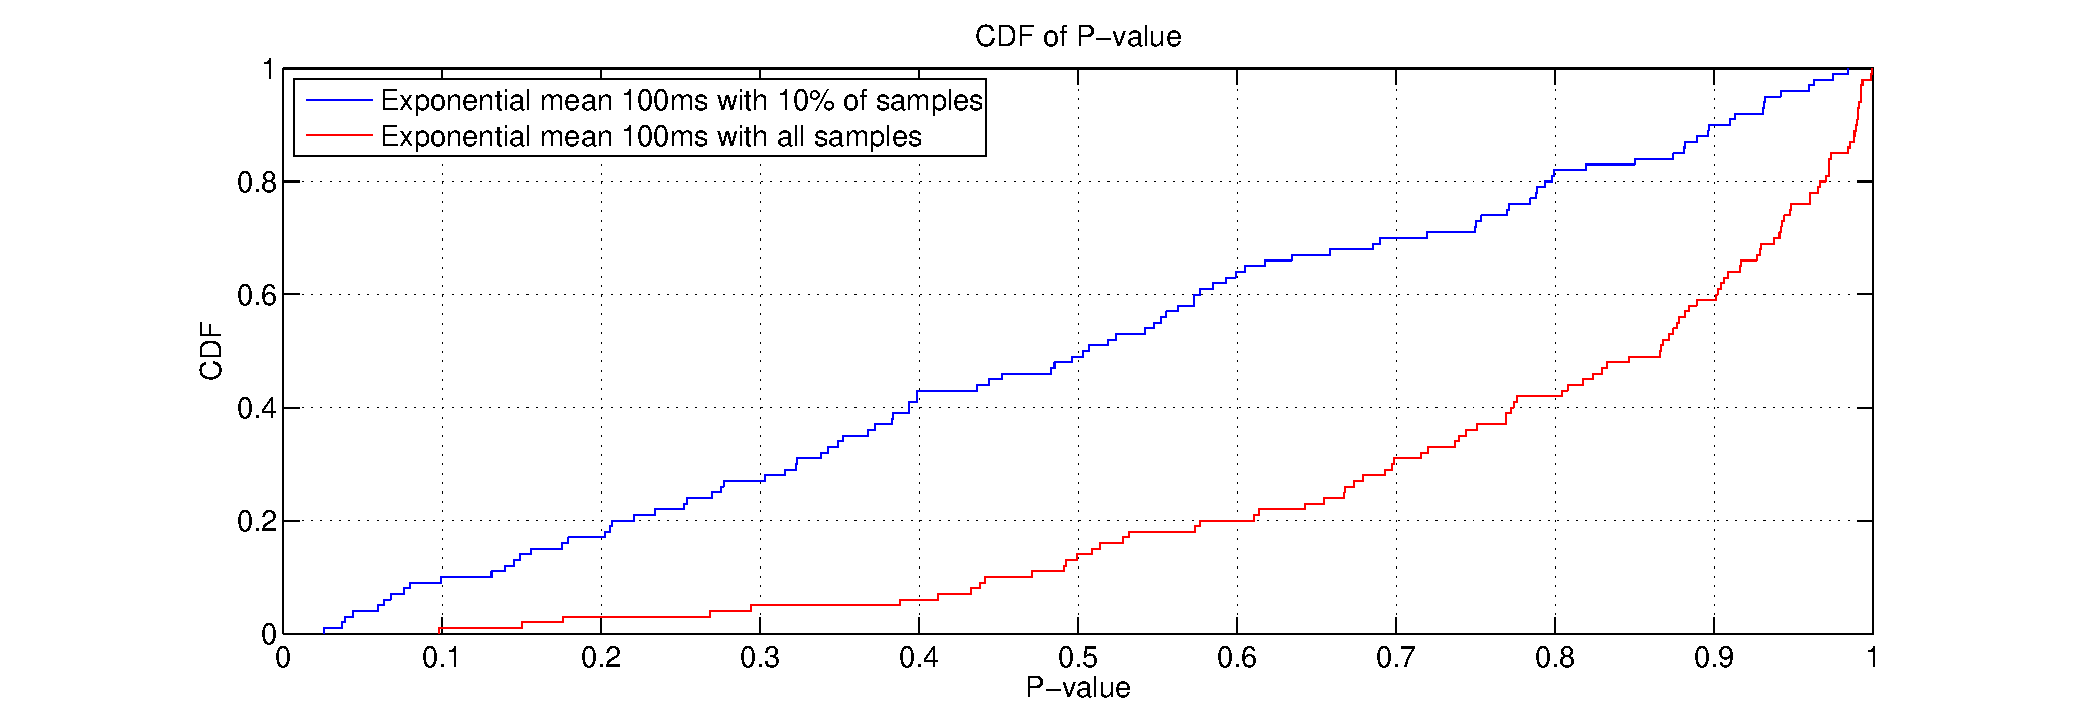
\includegraphics[width=0.9\textwidth, trim = 0mm 0mm 0mm 0mm, clip]{../images/results/GlobalView/KS/ks_optimization/pvalue_exponential100ms}
	\end{figure}
\end{frame}

\subsubsection*{Session and in-Session experiments}
\begin{frame}[c]
	\frametitle{Session number experiment}
	Test the effect of the number of sessions in the estimation process and KS. \\
	Fixed configuration for session and flow levels. Packet size and inter-arrivals are randomized.
	\begin{columns}
		\centering
		\column{.33\textwidth}
		\begin{figure}
			\centering
			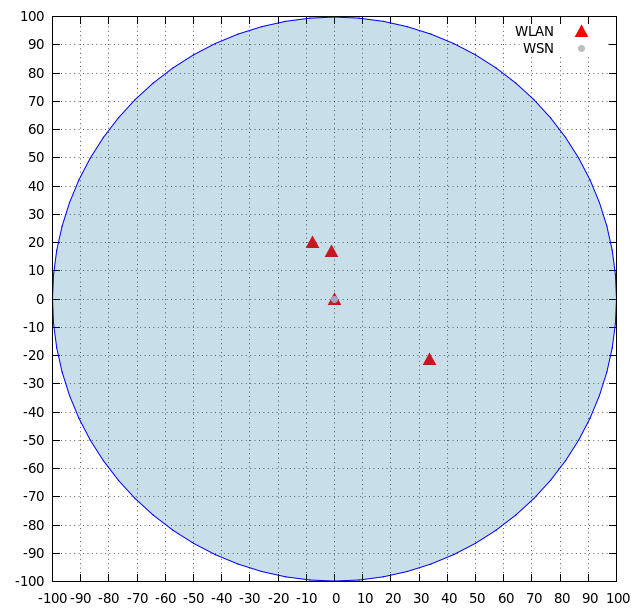
\includegraphics[width=0.9\textwidth]{../images/results/GlobalView/sessions/3sessions}
		\end{figure}
		\column{.33\textwidth}
		\begin{figure}
			\centering
			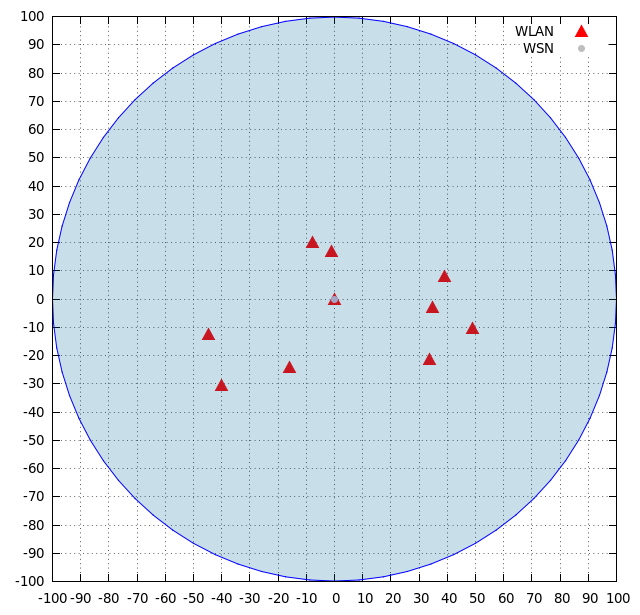
\includegraphics[width=0.9\textwidth]{../images/results/GlobalView/sessions/9sessions}
		\end{figure}
		\column{.33\textwidth}
		\begin{figure}
			\centering
			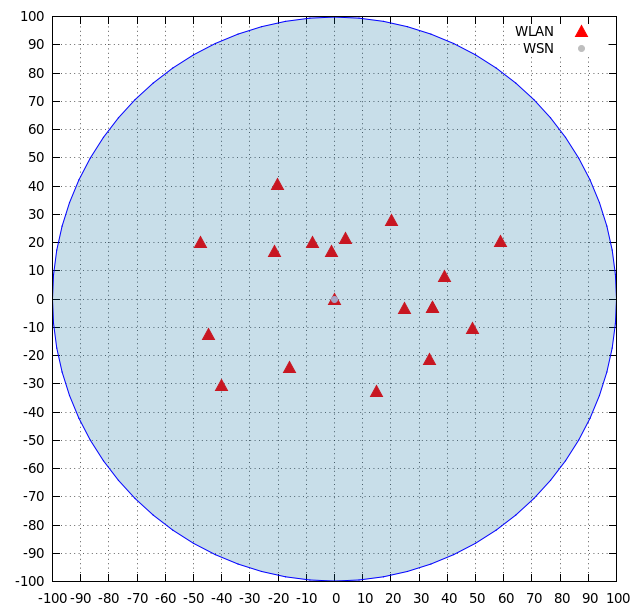
\includegraphics[width=0.9\textwidth]{../images/results/GlobalView/sessions/18sessions}
		\end{figure}
	\end{columns}
	
	\scriptsize
	\begin{table}
	\centering
		\begin{tabular}{ c | c | c || c | c || c | c }
			& \multicolumn{2}{ c || }{3 sessions} &  \multicolumn{2}{ c || }{9 sessions} & \multicolumn{2}{ c }{18 sessions}\\ \hline \hline
			& Mean & Std. Dev. & Mean & Std. Dev. & Mean & Std. Dev. \\ \hline
			$\xi$ & 0.184869 & 0.0109214 & 0.0639 & 0.0095 & 0.025 & 0.0097 \\ 
			$\sigma$ & 0.00337252 & 4.80725e-05 & 0.0036 & 5.9426e-05 & 0.0045 & 6.27E-005 \\
			$p$ & 0.38928 & 0.00444004 & 0.2996 & 0.0057 & 0.2397 & 0.004 \\
			$p-value$ & 0.525856 & 0 0.253306 & 0.6874 & 0.2693 & 0.796 & 0.1874 \\ \hline
			$Fail$ & \multicolumn{2}{ c || }{0 \%} &  \multicolumn{2}{ c || }{0 \%} & \multicolumn{2}{ c }{0 \%}\\
		\end{tabular}
	\end{table}
\end{frame}

\begin{frame}[c]
	\frametitle{In-Session Experiment}
	\begin{itemize}
		\item 10 WLAN users. Flow and packet levels are randomized.
		\item Two load cases:
		\begin{itemize}
			\item Load range of 20\% - 45\%.
			\item Load range of 35\% - 65\%.
		\end{itemize}
	\end{itemize}
	
	\begin{columns}
		\centering
		\column{.5\textwidth}
		\begin{figure}
			\centering
			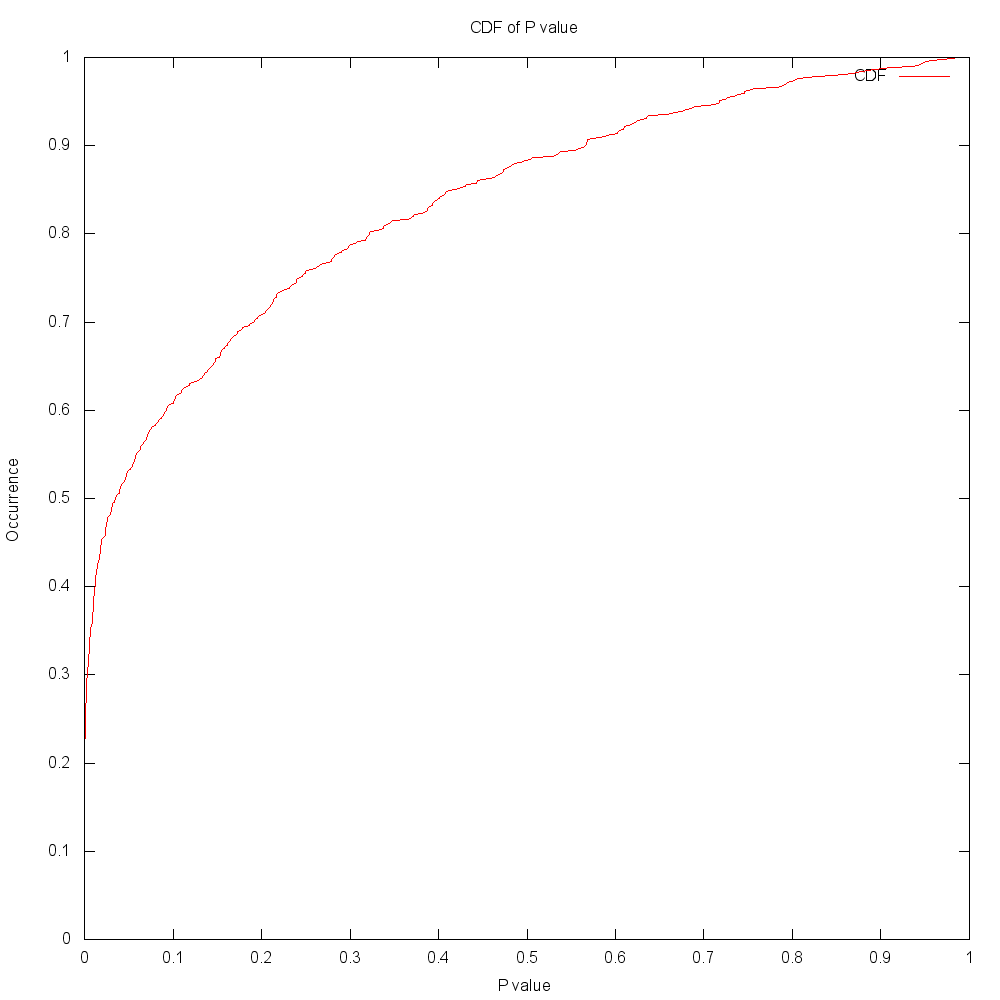
\includegraphics[width=1\textwidth]{../images/results/GlobalView/flows/limited_load/cdf_p}
		\end{figure}
		\column{.5\textwidth}
		\begin{figure}
			\centering
			\includegraphics[width=1\textwidth]{../images/results/GlobalView/flows/limited_load/nflows}
		\end{figure}
	\end{columns}
	
	\begin{columns}
		\centering
		\column{.5\textwidth}
		\begin{figure}
			\centering
			\includegraphics[width=1\textwidth]{../images/results/GlobalView/flows/limited_load/samples}
		\end{figure}
		\column{.5\textwidth}
		\begin{figure}
			\centering
			\includegraphics[width=1\textwidth]{../images/results/GlobalView/flows/limited_load/load}
		\end{figure}
	\end{columns}
\end{frame}

\subsubsection*{Autocorrelation study of the time sequence of sources of activity in the WLAN}
\begin{frame}[c]
	\frametitle{Autocorrelation study of the time sequence of sources of activity in the WLAN}
\end{frame}

%Local View
\subsection{Local View}
\begin{frame}[c]
	\frametitle{Local View Experiments}
	\begin{itemize}
		\item Autocorrelation of the IN/OUT sequence of DATA packets
		\item Density study of the consecutive skipped Active periods
	\end{itemize}
\end{frame}

\subsubsection*{Autocorrelation of the IN/OUT sequence of DATA packets}

\begin{frame}[c]
	\frametitle{Autocorrelation of the IN/OUT sequence of DATA packets}
	\begin{itemize}
		\item The consecutive active WLAN periods are independent and generated from independent WLAN users.
		\item The active periods should be independent.
		\item Generate a sequence of IN/OUT to study the autocorrelation.
	\end{itemize}
	
	\begin{columns}
		\column{.4\textwidth}
		\begin{figure}
			\centering
			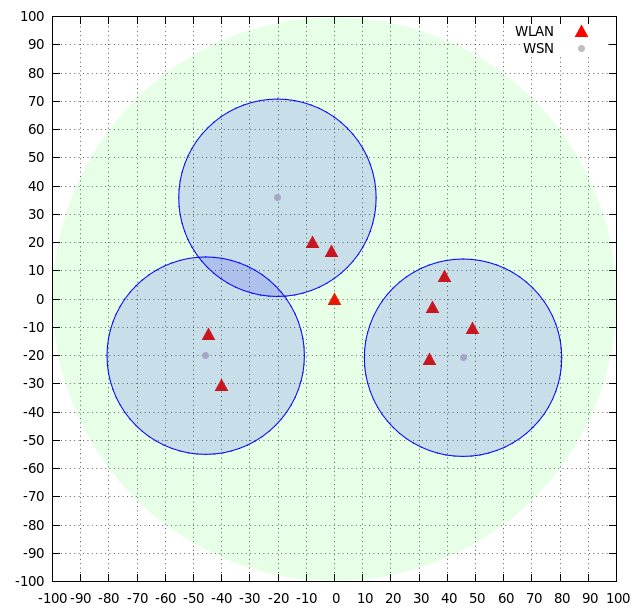
\includegraphics[width=0.5\textwidth]{../images/results/autocorrelation/localview/8sessions}
		\end{figure}
		\begin{figure}
			\centering
			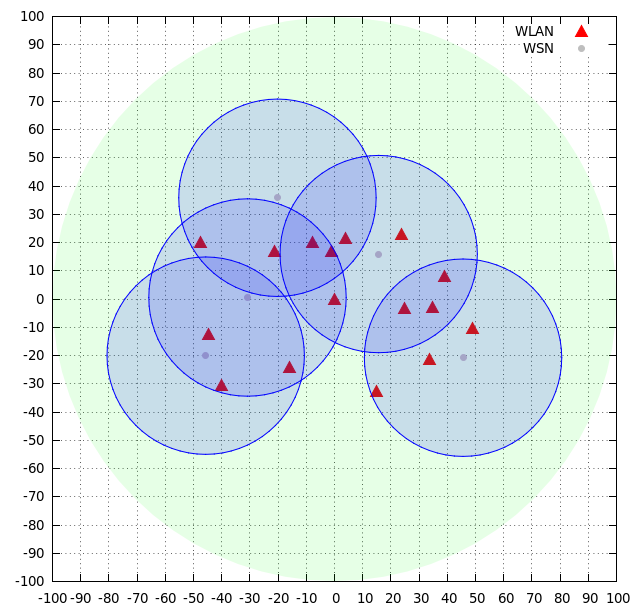
\includegraphics[width=0.5\textwidth]{../images/results/autocorrelation/localview/15sessions}
		\end{figure}
		
		\column{.6\textwidth}
		\begin{columns}
			\column{.333\textwidth}
			\begin{figure}
				\centering
				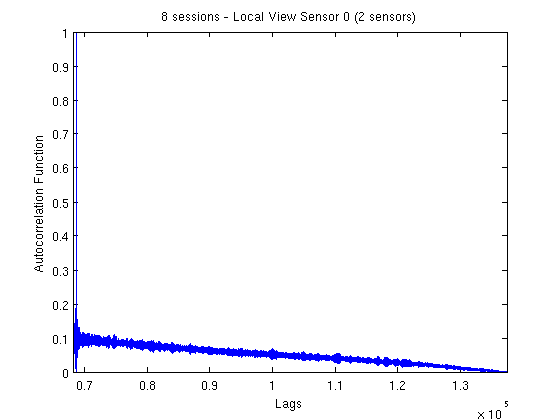
\includegraphics[width=0.9\textwidth]{../images/results/autocorrelation/localview/8sessions_sensor0}
			\end{figure}
			\column{.333\textwidth}
			\begin{figure}
				\centering
				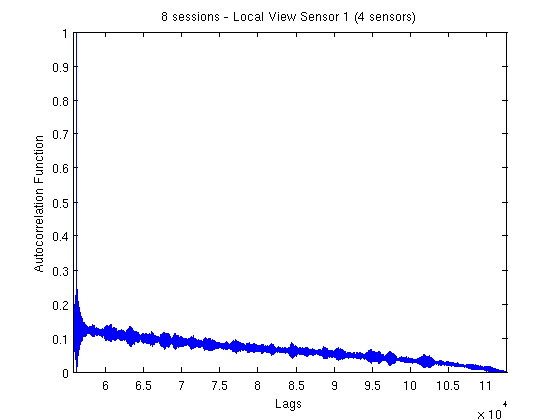
\includegraphics[width=0.9\textwidth]{../images/results/autocorrelation/localview/8sessions_sensor1}
			\end{figure}
			\column{.333\textwidth}
			\begin{figure}
				\centering
				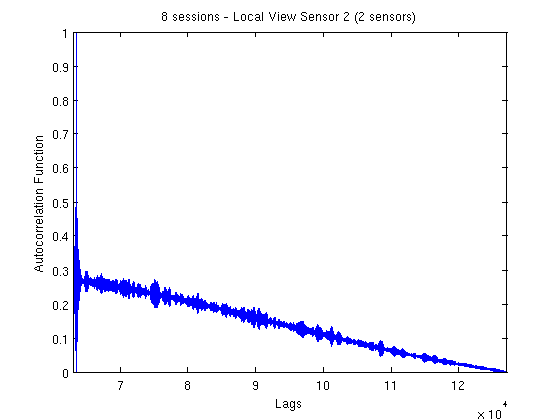
\includegraphics[width=0.9\textwidth]{../images/results/autocorrelation/localview/8sessions_sensor2}
			\end{figure}
		\end{columns}
		
		\begin{columns}
			\column{.333\textwidth}
			\begin{figure}
				\centering
				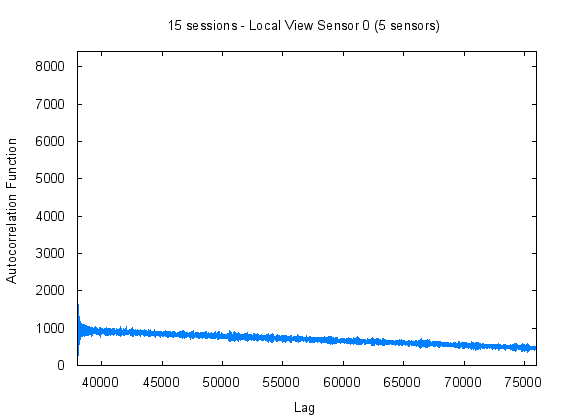
\includegraphics[width=0.9\textwidth]{../images/results/autocorrelation/localview/15sessions_sensor0}
			\end{figure}
			\column{.333\textwidth}
			\begin{figure}
				\centering
				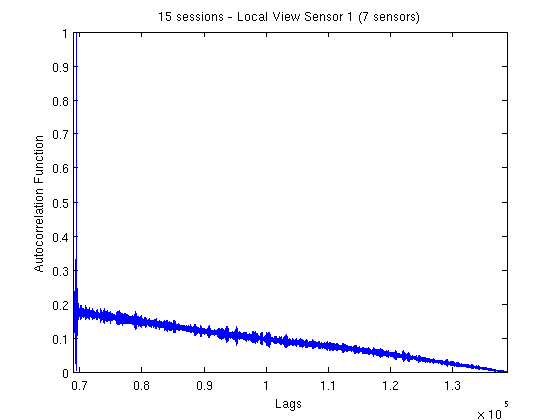
\includegraphics[width=0.9\textwidth]{../images/results/autocorrelation/localview/15sessions_sensor1}
			\end{figure}
			\column{.333\textwidth}
			\begin{figure}
				\centering
				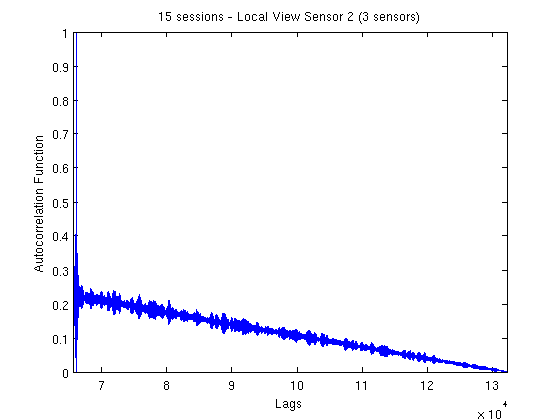
\includegraphics[width=0.9\textwidth]{../images/results/autocorrelation/localview/15sessions_sensor2}
			\end{figure}
		\end{columns}
		
		\begin{columns}
			\column{.333\textwidth}
			\begin{figure}
				\centering
				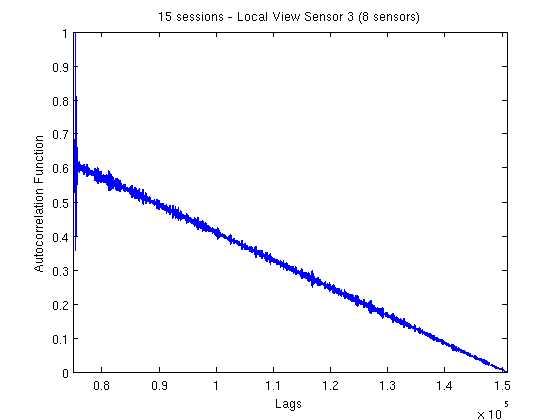
\includegraphics[width=0.9\textwidth]{../images/results/autocorrelation/localview/15sessions_sensor3}
			\end{figure}
			\column{.333\textwidth}
			\begin{figure}
				\centering
				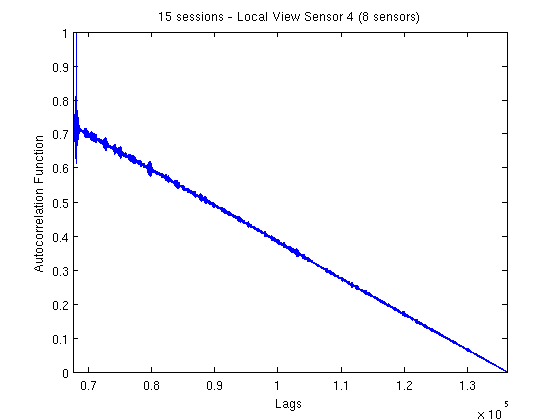
\includegraphics[width=0.9\textwidth]{../images/results/autocorrelation/localview/15sessions_sensor4}
			\end{figure}
		\end{columns}
		
	\end{columns}
\end{frame}

\subsubsection*{Density study of the consecutive skipped Active periods in Local View}
\begin{frame}[c]
	\frametitle{Density study of the consecutive skipped Active periods in Local View}
	\begin{itemize}
		\item Generate a sequence of \underline{consecutive} skipped active periods for the sensor.
		\item The sequence follows a Geometric Distribution.
		\item Geometric Distribution characterized by a single parameter $p$:
	\end{itemize}
	\begin{equation}
		p = \frac{1}{1+E(x)}
	\end{equation}
	\begin{itemize}
		\item Generation of the estimated Geometric Distribution:
	\end{itemize}
	\begin{equation}
		CDF(k) = 1-(1-p)^{k+1}
	\end{equation}
	\begin{figure}
		\centering
		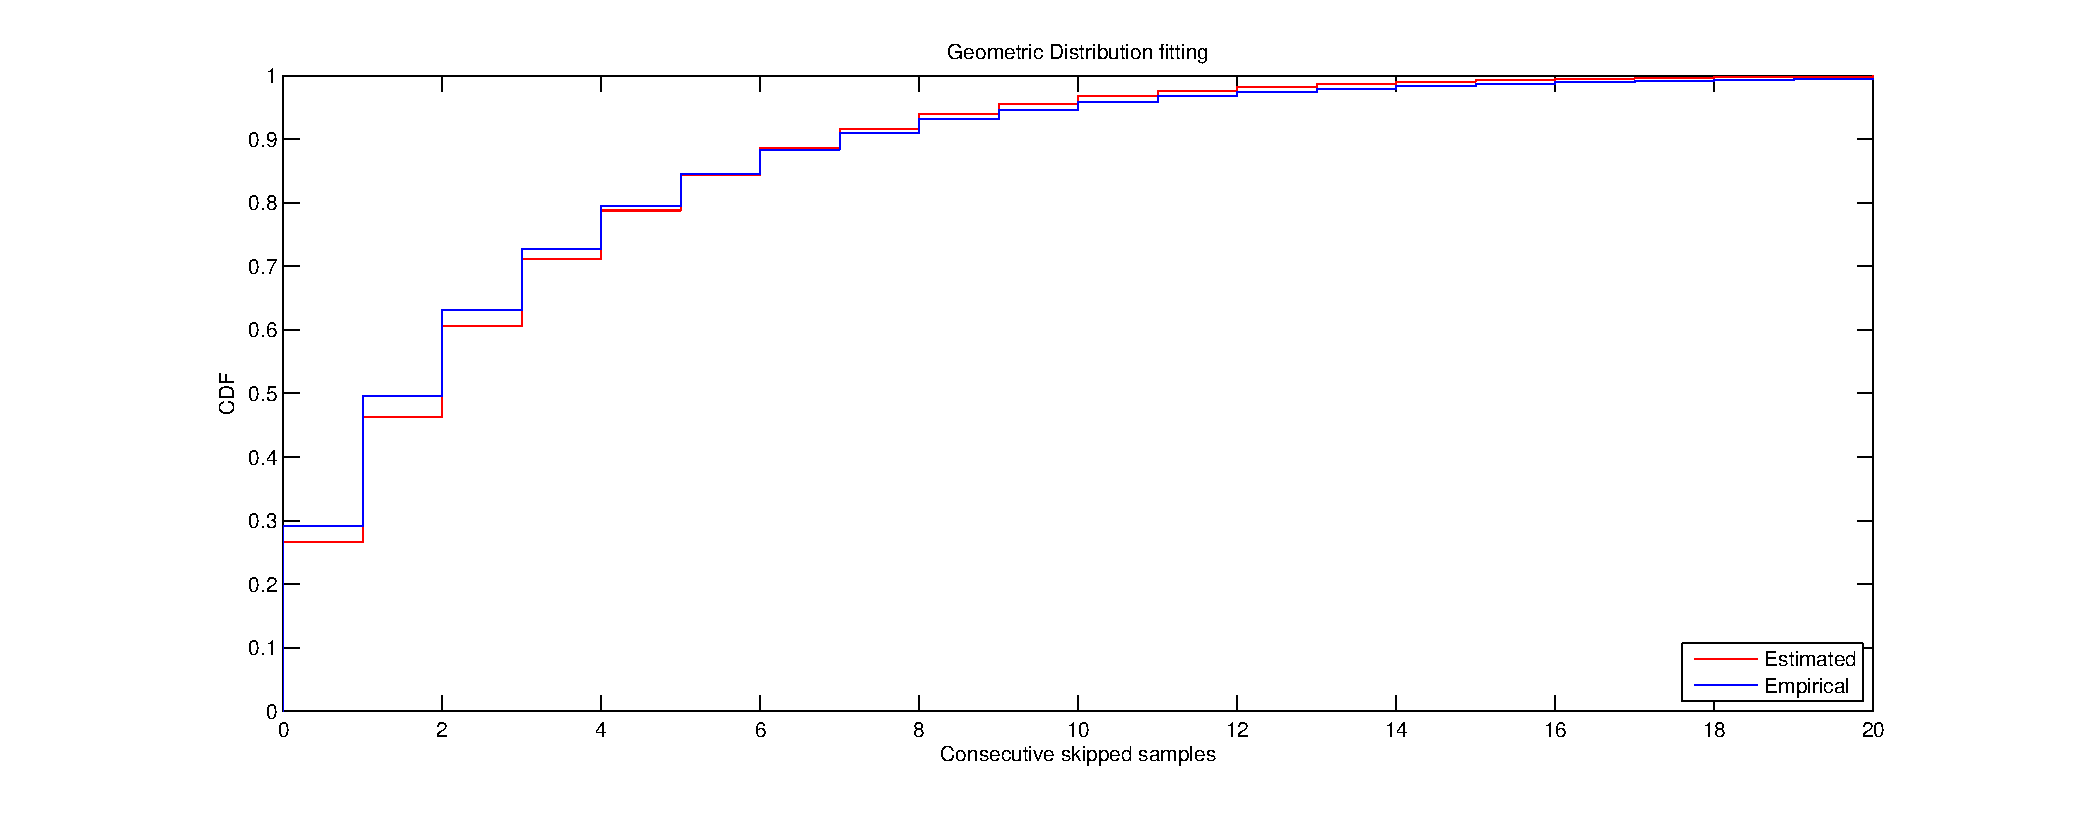
\includegraphics[width=0.8\textwidth]{../images/results/autocorrelation/localview/geometric}
	\end{figure}
\end{frame}

\begin{frame}[c]
	\frametitle{Goodness-of-fit test for Geometric Distribution}
	\begin{itemize}
		\item Geometric Distribution is discrete.
		\item Kolmogorov-Smirnov cannot be applyied to discrete distributions.
		\item Two solutions: Mean-Square Error and Chi-squared validation test.
	\end{itemize}
	Mean-square Error:
	\begin{equation}
		\sum_{k=0}^{\infty}[P_{geometric}(k) - P_{empirical}(k)]^2
	\end{equation}
	
	\begin{columns}
		\column{.333\textwidth}
		\begin{figure}
			\centering
			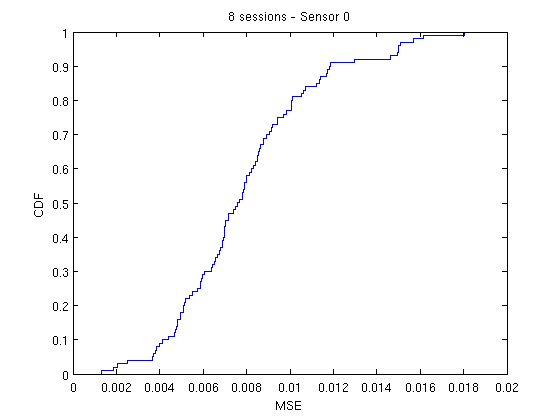
\includegraphics[width=\textwidth]{../images/results/autocorrelation/localview/mse/8sessions_mse_sensor0}
		\end{figure}
		\column{.333\textwidth}
		\begin{figure}
			\centering
			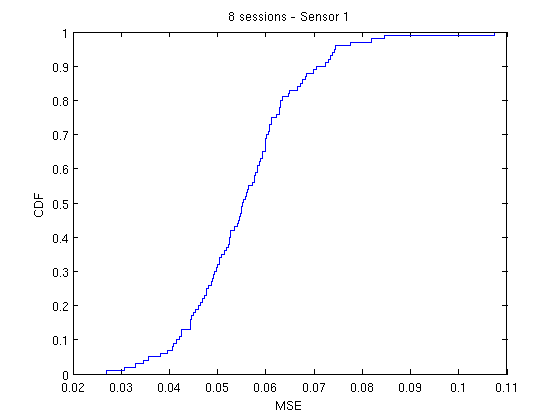
\includegraphics[width=1\textwidth]{../images/results/autocorrelation/localview/mse/8sessions_mse_sensor1}
		\end{figure}
		\column{.333\textwidth}
		\begin{figure}
			\centering
			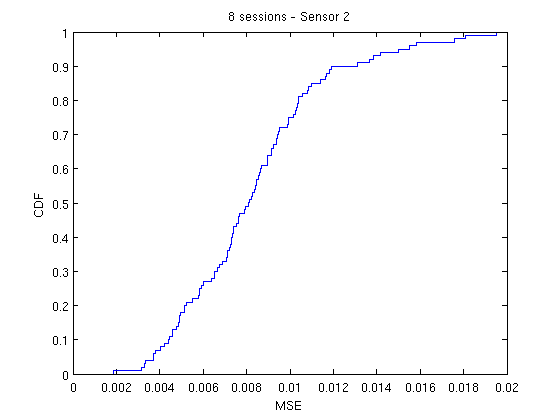
\includegraphics[width=1\textwidth]{../images/results/autocorrelation/localview/mse/8sessions_mse_sensor2}
		\end{figure}
	\end{columns}
\end{frame}

\begin{frame}
	\frametitle{Goodness-of-fit test for Geometric Distribution}
	Chi-squared validation test:
	
	\begin{columns}
		\column{.5\textwidth}
		\begin{figure}
			\centering
			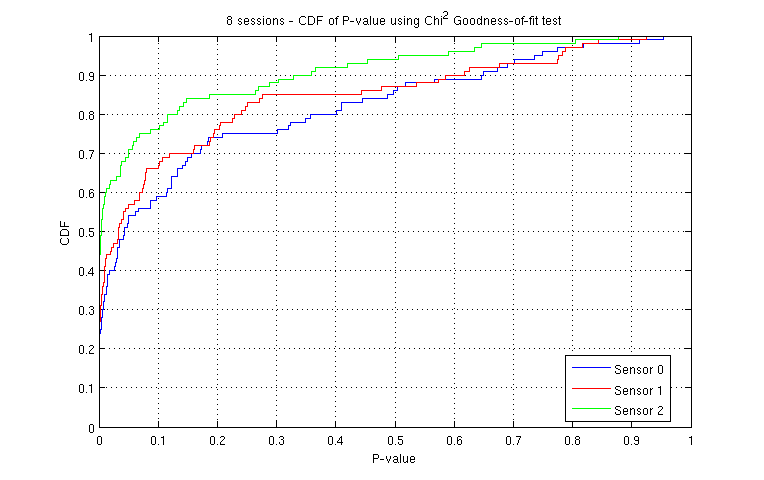
\includegraphics[width=1\textwidth]{../images/results/autocorrelation/localview/chi2/8sessions_cdf_p}
		\end{figure}
		\column{.5\textwidth}
		\begin{figure}
			\centering
			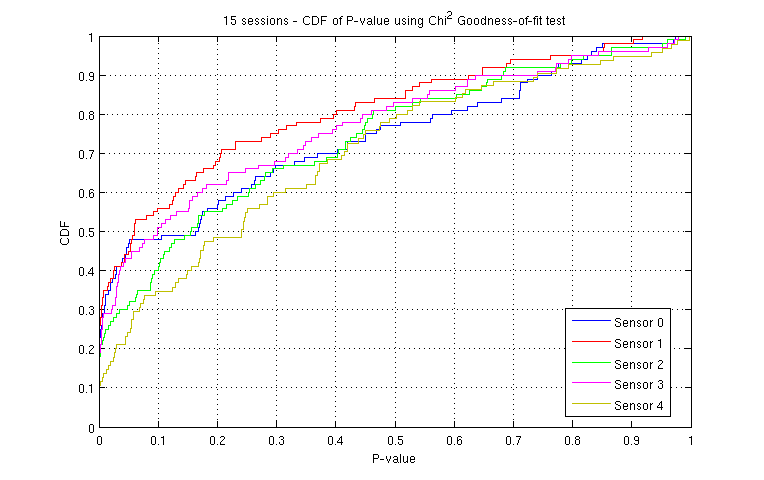
\includegraphics[width=1\textwidth]{../images/results/autocorrelation/localview/chi2/15sessions_cdf_p}
		\end{figure}
	\end{columns}
\end{frame}

%References
\section{References}

\begin{frame}[allowframebreaks]
  \frametitle<presentation>{Weiterf¸hrende Literatur}    
  \begin{thebibliography}{10}    
  \beamertemplatebookbibitems
  \bibitem{Autor1990}
    A.~Autor.
    \newblock {\em Einf¸hrung in das Pr‰sentationswesen}.
    \newblock Klein-Verlag, 1990.
  \beamertemplatearticlebibitems
  \bibitem{Jemand2000}
    S.~Jemand.
    \newblock On this and that.
    \newblock {\em Journal of This and That}, 2(1):50--100, 2000.
  \end{thebibliography}
\end{frame}

\end{document}